\section[پروژه دوم - تشخیص چهره با PCA]{\faUserShield\ \ پروژه دوم - تشخیص چهره با الگوریتم PCA}

\begin{stepbox}

\field{۱. آماده‌سازی و بارگذاری داده‌ها \lr{(Load Data)}}{
در این پروژه قصد داریم از الگوریتم \lr{Principal Component Analysis (PCA)} برای استخراج ویژگی‌های پنهان تصاویر چهره و بازسازی آن‌ها استفاده کنیم. دیتاست مورد استفاده شامل تصاویر چهره افراد در دو حالت طبیعی و خندان است. 
در گام نخست، تصاویر خوانده شده و برای بررسی صحت بارگذاری، تعدادی از آن‌ها رسم شدند.

\vspace{0.4cm}
\begin{center}
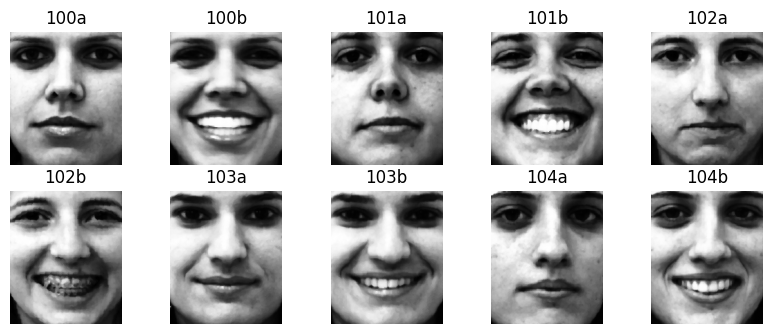
\includegraphics[width=.7\textwidth]{images/dataset_samples.png}
\captionof{figure}{نمونه‌ای از تصاویر چهره‌ی بارگذاری شده از مجموعه داده}
\label{fig:dataset_samples}
\end{center}

الگوریتم \lr{PCA} برای انجام عملیات جبر خطی نیازمند داده‌های برداری است. بنابراین، هر تصویر دوبعدی با ابعاد $193 \times 162$ پیکسل، به یک بردار ستونی تک‌بعدی (\lr{Flatten}) با طول $D = 31266$ تبدیل گردید. 
با قرار دادن ۱۹۰ تصویر اول (مربوط به چهره‌های طبیعی) در کنار یکدیگر، ماتریس کل دادگان با نام $\Gamma$ تشکیل شد:
\[
\Gamma = \begin{bmatrix} | & | & & | \\ \Gamma_1 & \Gamma_2 & \dots & \Gamma_{190} \\ | & | & & | \end{bmatrix} \in \mathbb{R}^{31266 \times 190}
\]
بهینه‌سازی پیاده‌سازی: برای جلوگیری از افت عملکرد (\lr{Performance Drop}) ناشی از تخصیص پویای حافظه در حلقه‌ها هنگام کار با کتابخانه \lr{NumPy}، از روش پیش‌تخصیص حافظه (\lr{Pre-allocation}) با استفاده از تابع \lr{\texttt{np.empty}} استفاده گردید تا ماتریس دادگان با بالاترین سرعت ممکن تشکیل شود.
}
\newpage
\field{۲. محاسبه تصویر میانگین \lr{(Mean Image)} و نرمال‌سازی}{
الگوریتم \lr{PCA} به دنبال یافتن جهت‌های بیشترین واریانس است. بدین منظور، مبدأ مختصات فضای داده‌ها باید دقیقاً در مرکز آن‌ها قرار گیرد. لذا ابتدا بردار «چهره میانگین» ($\Psi$) با میانگین‌گیری روی تمامی ۱۹۰ تصویر محاسبه شد:
\[
\Psi = \frac{1}{n}\sum_{i=1}^{n} \Gamma_i
\]

\vspace{0.4cm}
\begin{center}
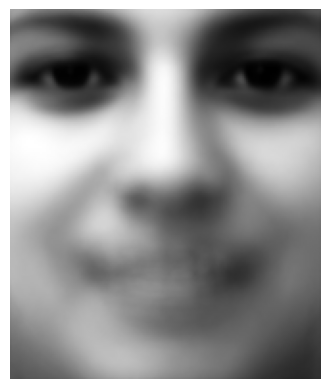
\includegraphics[width=.35\textwidth]{images/mean_face.png}
\captionof{figure}{تصویر چهره میانگین ($\Psi$) محاسبه شده از ۱۹۰ چهره‌ی حالت طبیعی}
\label{fig:mean_face}
\end{center}

سپس با کسر کردن این چهره میانگین از تک‌تک بردارهای تصاویر ($\Phi_i = \Gamma_i - \Psi$)، ماتریس داده‌های نرمال‌شده ($A$) تشکیل گردید که در مراحل بعدی به عنوان ورودی اصلی الگوریتم مورد استفاده قرار می‌گیرد.
}

\field{۳. ماتریس کوواریانس و استخراج چهره‌های ویژه \lr{(Covariance Trick \& Eigenfaces)}}{
برای یافتن جهت‌های بیشترین تغییرات، باید مقادیر ویژه و بردارهای ویژه‌ی ماتریس کوواریانس $C = A A^T$ محاسبه می‌شد. اما با توجه به ابعاد ماتریس $A$ (که برابر با $31266 \times 190$ است)، ماتریس $C$ ابعادی برابر با $31266 \times 31266$ خواهد داشت که محاسبه‌ی مقادیر ویژه‌ی آن از نظر محاسباتی و حافظه تقریباً غیرممکن است.

برای حل این چالش، از ترفند ریاضی ماتریس کوواریانس استفاده شد. به جای ماتریس بزرگ $C$، ماتریس بسیار کوچک‌تر $L = A^T A$ با ابعاد $190 \times 190$ تشکیل گردید. از نظر جبری ثابت می‌شود که اگر $v$ بردار ویژه‌ی ماتریس $L$ با مقدار ویژه‌ی $\lambda$ باشد:
\begin{align*}
(A^T A) v = \lambda v &\implies A (A^T A) v = A (\lambda v) \\
&\implies (A A^T) (Av) = \lambda (Av) \\
&\implies C (Av) = \lambda (Av)
\end{align*}
طبق این اثبات، با ضرب بردارهای ویژه‌ی ماتریس کوچک $L$ در ماتریس داده‌ها ($A$)، بردارهای ویژه‌ی ماتریس اصلی ($U = Av$) به دست می‌آیند. در نهایت، برای ایجاد یک پایه‌ی یکّه و متعامد \lr{(Orthonormal Basis)}، ستون‌های ماتریس $U$ بر اندازه خود \lr{(L2-Norm)} تقسیم شدند.

پس از استخراج، مقادیر ویژه به صورت نزولی مرتب شدند. نمودار زیر نشان می‌دهد که بخش عمده‌ی واریانس (اطلاعات) داده‌ها تنها در تعداد محدودی از مؤلفه‌های اصلی ابتدایی نهفته است.

\vspace{0.4cm}
\begin{center}
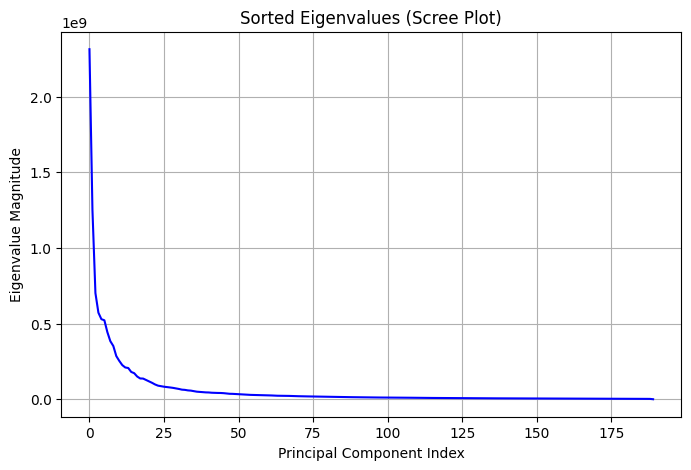
\includegraphics[width=.5\textwidth]{images/scree_plot.png}
\captionof{figure}{نمودار مقادیر ویژه مرتب‌شده \lr{(Scree Plot)} که میزان اطلاعات هر مؤلفه را نشان می‌دهد}
\label{fig:scree_plot}
\end{center}

با تغییر شکل \lr{(Reshape)} بردارهای ویژه‌ی استخراج‌شده به ابعاد تصویر اولیه، تصاویری موسوم به «چهره‌های ویژه» \lr{(Eigenfaces)} به دست می‌آیند. در شکل زیر ۵ بردار ویژه‌ی برتر که بیشترین واریانس داده‌ها را در بر دارند، نمایش داده شده‌اند.

\vspace{0.4cm}
\begin{center}
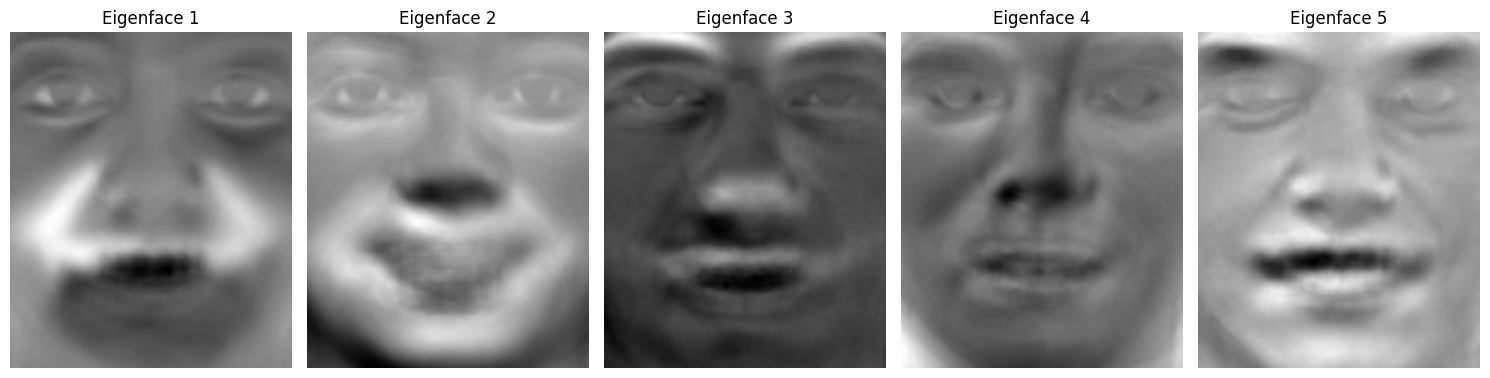
\includegraphics[width=.85\textwidth]{images/eigenfaces_top5.png}
\captionof{figure}{پنج چهره‌ی پایه‌ی برتر \lr{(Top 5 Eigenfaces)} استخراج‌شده از ماتریس کوواریانس}
\label{fig:eigenfaces_top5}
\end{center}
}

\field{۴. بازسازی تصاویر \lr{(Image Reconstruction)}}{
برای بازسازی یک تصویر، ابتدا باید آن را روی فضای جدیدِ ساخته‌شده توسط چهره‌های پایه تصویر \lr{(Project)} کنیم تا وزن‌های ترکیب خطی به دست آیند. فرض کنید $U_K$ ماتریسی شامل $K$ بردار ویژه‌ی برتر باشد و $\Phi$ تصویر نرمال‌شده‌ی ورودی باشد:
\[
W = U_K^T \Phi
\]
ماتریس $W$ نشان‌دهنده‌ی وزن‌هایی است که مشخص می‌کند تصویر ورودی چه مقدار از هر چهره‌ی پایه را در خود دارد. سپس با ضرب این وزن‌ها در چهره‌های پایه و افزودن چهره‌ی میانگین ($\Psi$)، تصویر بازسازی‌شده ($\Gamma_{rec}$) به فضای پیکسلی اولیه بازگردانده می‌شود:
\[
\Gamma_{rec} = (U_K W) + \Psi
\]

شکل زیر مقایسه‌ای بین چهره‌ی اصلی و چهره‌ی بازسازی‌شده را نشان می‌دهد. عملکرد موفقیت‌آمیز الگوریتم در حفظ ساختار کلی چهره (با وجود کاهش شدید ابعاد داده‌ها) کاملاً مشهود است.

\vspace{0.4cm}
\begin{center}
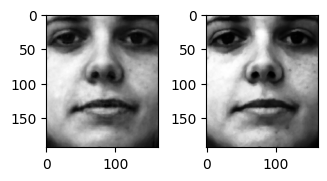
\includegraphics[width=.6\textwidth]{images/recon_single.png}
\captionof{figure}{مقایسه تصویر اصلی (راست) و تصویر بازسازی‌شده با استفاده از بردارهای ویژه (چپ)}
\label{fig:recon_single}
\end{center}
}

\newpage
\field{۵. تحلیل اثر تعداد مؤلفه‌های اصلی بر کیفیت بازسازی \lr{(Trade-off Analysis)}}{
در این بخش، هدف بررسی موازنه \lr{(Trade-off)} میان میزان فشرده‌سازی اطلاعات و خطای بازسازی تصویر است. بدین منظور، یک تصویر به صورت تصادفی از مجموعه داده‌های آموزشی انتخاب گردید و عملیات بازسازی به ازای تمامی مقادیر ممکن برای تعداد چهره‌های پایه ($1 \le K \le 190$) روی آن انجام شد. 

با محاسبه‌ی میانگین مربعات خطا \lr{(MSE)} برای هر حالت، کمترین و بیشترین میزان خطا استخراج گردید. از نظر ریاضی، زمانی که از تنها یک بردار ویژه ($K=1$) استفاده شود، بیشترین اطلاعات دور ریخته شده و خطا \lr{Max} خواهد بود. در مقابل، زمانی که $K=190$ باشد، از آنجا که تمام فضای ویژگی حفظ شده است، بازسازی باید بدون نقص باشد و خطای \lr{MSE} به کمترین حد خود (نزدیک به صفر) می‌رسد.
نمودار زیر روند نزولی \lr{MSE} را با افزایش $K$ نشان می‌دهد.

\vspace{0.4cm}
\begin{center}
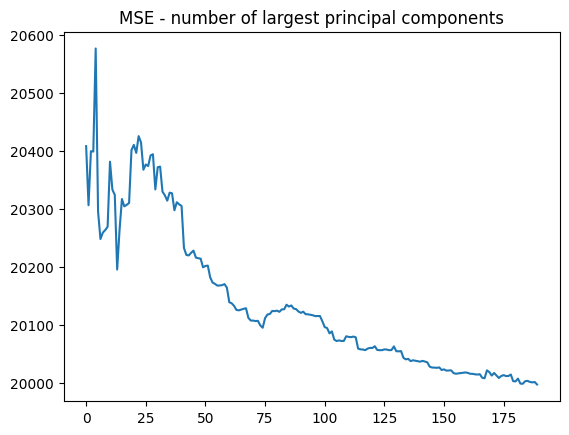
\includegraphics[width=.6\textwidth]{images/mse_vs_k.png}
\captionof{figure}{نمودار کاهش خطای بازسازی \lr{(MSE)} با افزایش تعداد مؤلفه‌های اصلی \lr{(K)}}
\label{fig:mse_vs_k}
\end{center}

برای درک بصری این پدیده، تصویر اصلی به همراه ۵ تصویر بازسازی‌شده با مقادیر مختلف $K$ (که کل محدوده‌ی چهره‌های پایه را پوشش می‌دهند) رسم شدند. همان‌طور که در شکل زیر پیداست، با $K=5$ تصویر حالتی شبح‌گونه دارد، اما با رسیدن به $K=50$، با وجود اینکه ابعاد داده از $31266$ به تنها $50$ عدد کاهش یافته است، چهره به خوبی قابل تشخیص است. این موضوع بیانگر قدرت بالای \lr{PCA} در فشرده‌سازی تصاویر \lr{(Image Compression)} می‌باشد.

\vspace{0.4cm}
\begin{center}
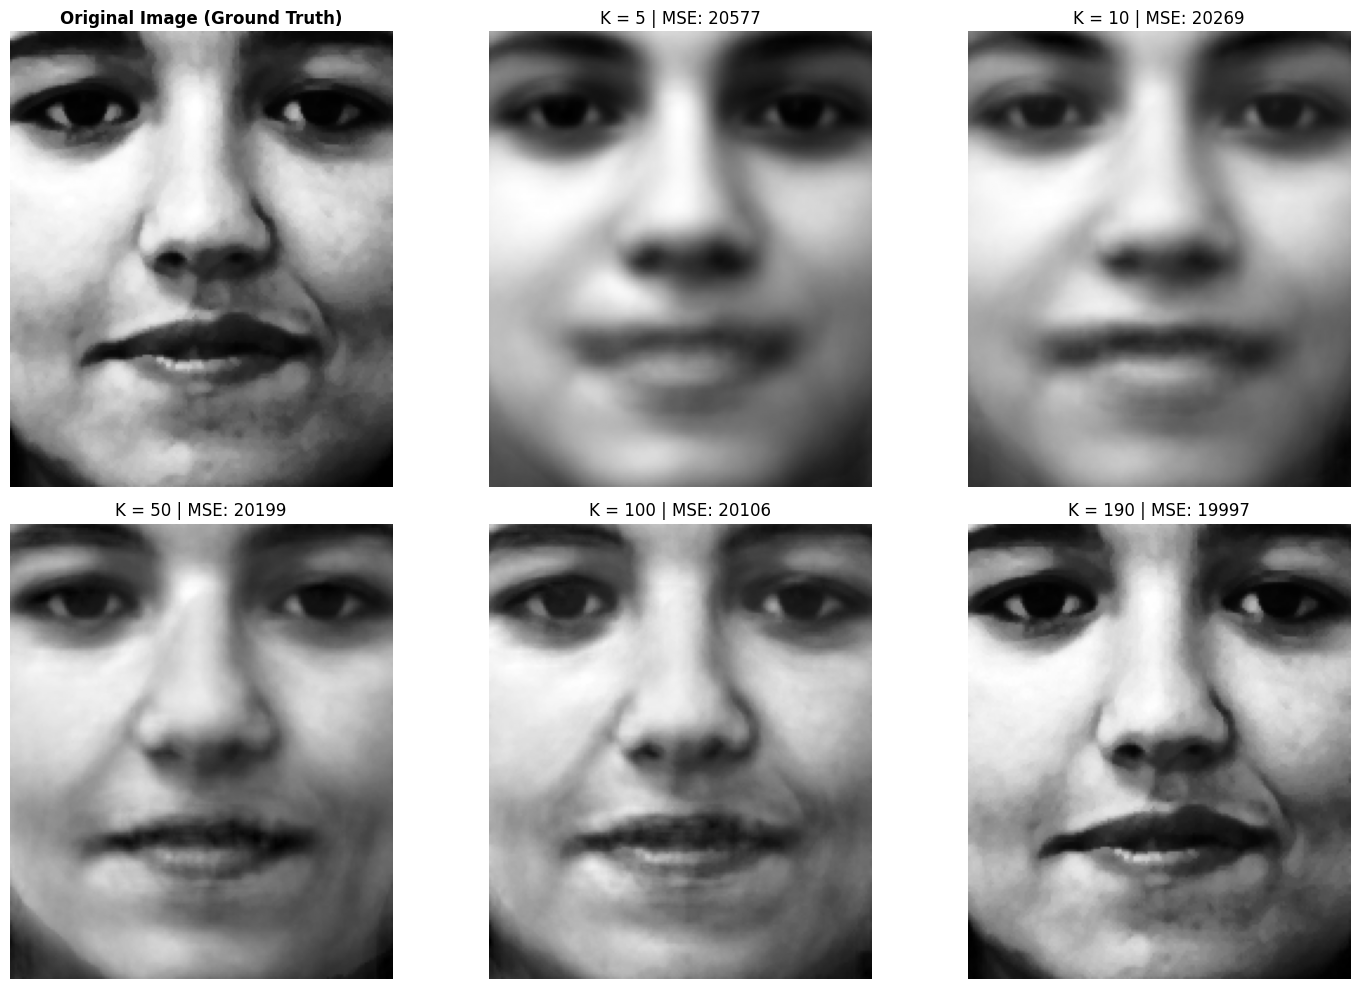
\includegraphics[width=.9\textwidth]{images/recon_grid_k.png}
\captionof{figure}{روند بهبود کیفیت تصویر بازسازی‌شده به ازای مقادیر مختلف $K$}
\label{fig:recon_grid_k}
\end{center}
}

\field{۶. ارزیابی مدل روی چهره‌های خندان \lr{(Smiling Images)}}{
تا به اینجا، فضای ویژگی \lr{(Face Space)} تنها با استفاده از چهره‌های با حالت طبیعی \lr{(Neutral)} ساخته شده بود. در این گام، یک چهره‌ی خندان از مجموعه داده انتخاب و بازسازی شد. 
نتایج نشان داد که اگرچه الگوریتم توانست ساختار کلی چهره را بازسازی کند، اما خطای \lr{MSE} نسبت به حالت چهره‌ی طبیعی کمی افزایش یافت. دلیل این امر آن است که تغییر حالت چهره به خندان، باعث جابجایی پیکسل‌های لب و چشم‌ها می‌شود و از آنجا که مدل \lr{PCA} ما روی داده‌های خنثی آموزش دیده است، در بازسازی دقیق این تغییراتِ خارج از وزیع آموزش \lr{(Out-of-Distribution)} کمی دچار خطا می‌گردد.

\vspace{0.4cm}
\begin{center}
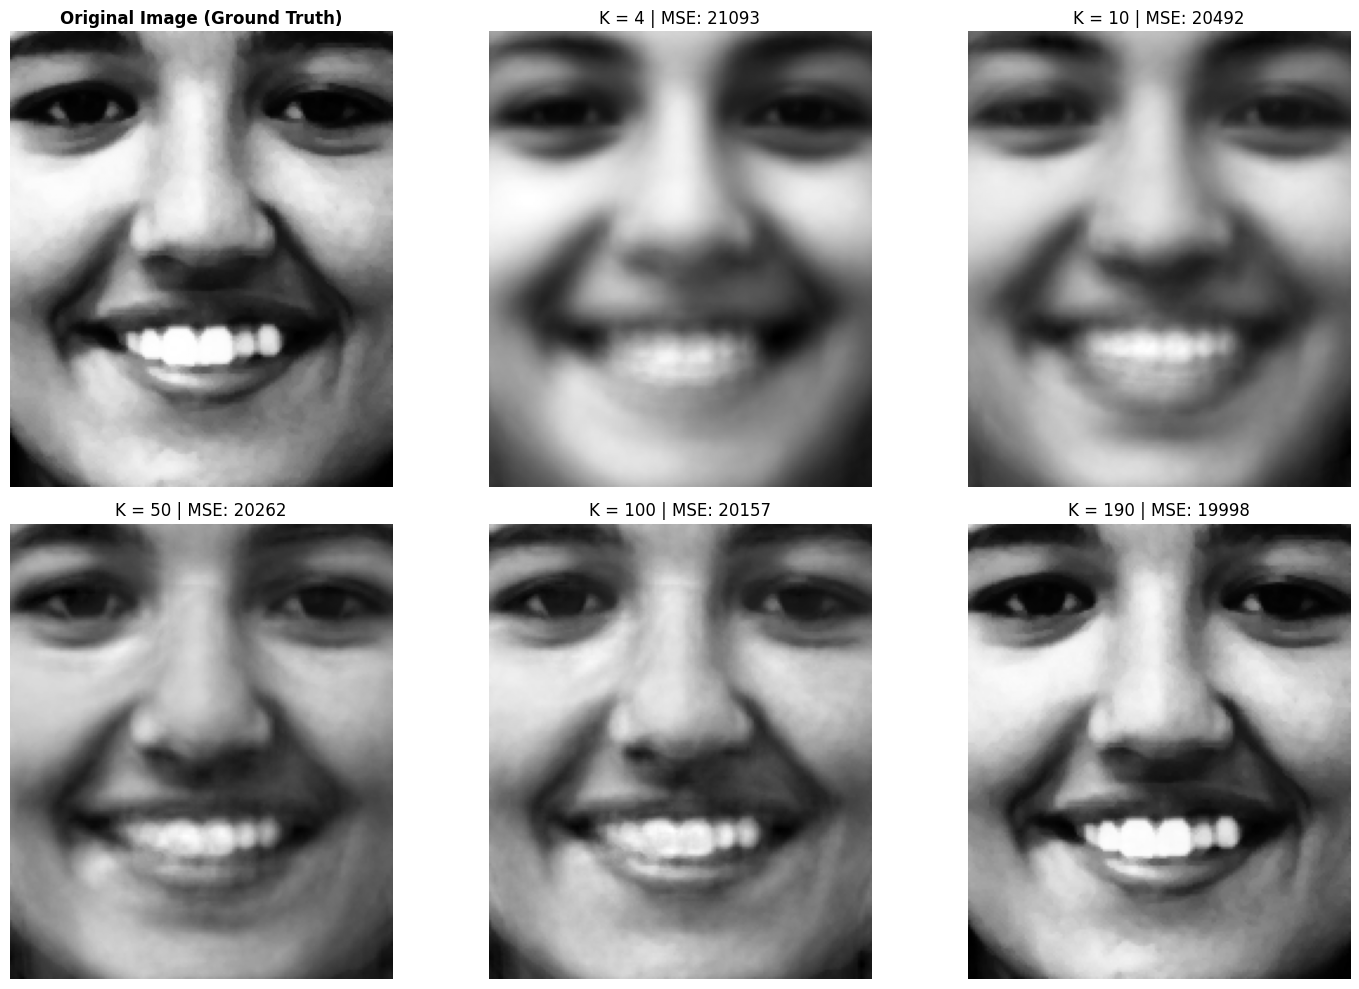
\includegraphics[width=.9\textwidth]{images/recon_grid_laugh.png}
\captionof{figure}{روند بازسازی یک چهره‌ی خندان با استفاده از مدل آموزش‌دیده روی چهره‌های طبیعی}
\label{fig:recon_grid_laugh}
\end{center}
}

\field{۷. ارزیابی روی داده‌های دیده نشده \lr{(Test Set)}}{
یکی از اصول اساسی یادگیری ماشین، ارزیابی مدل روی داده‌های جدید \lr{(Unseen Data)} است. برای این کار، ۱۰ عکس جدید که در فاز آموزش حضور نداشتند انتخاب شدند. 
نکته‌ی بسیار مهم ریاضی در این بخش، عدم محاسبه‌ی مجدد میانگین و بردارهای ویژه برای داده‌های تست است. تصاویر تست باید با استفاده از چهره‌ی میانگینِ فاز آموزش ($\Psi_{train}$) نرمال‌سازی شده و روی همان بردارهای ویژه‌ی قبلی تصویر \lr{(Project)} شوند. نتایج بازسازی نشان داد که الگوریتم \lr{Eigenfaces} دارای قدرت تعمیم‌پذیری \lr{(Generalization)} مناسبی برای چهره‌های جدید است.

\vspace{0.4cm}
\begin{center}
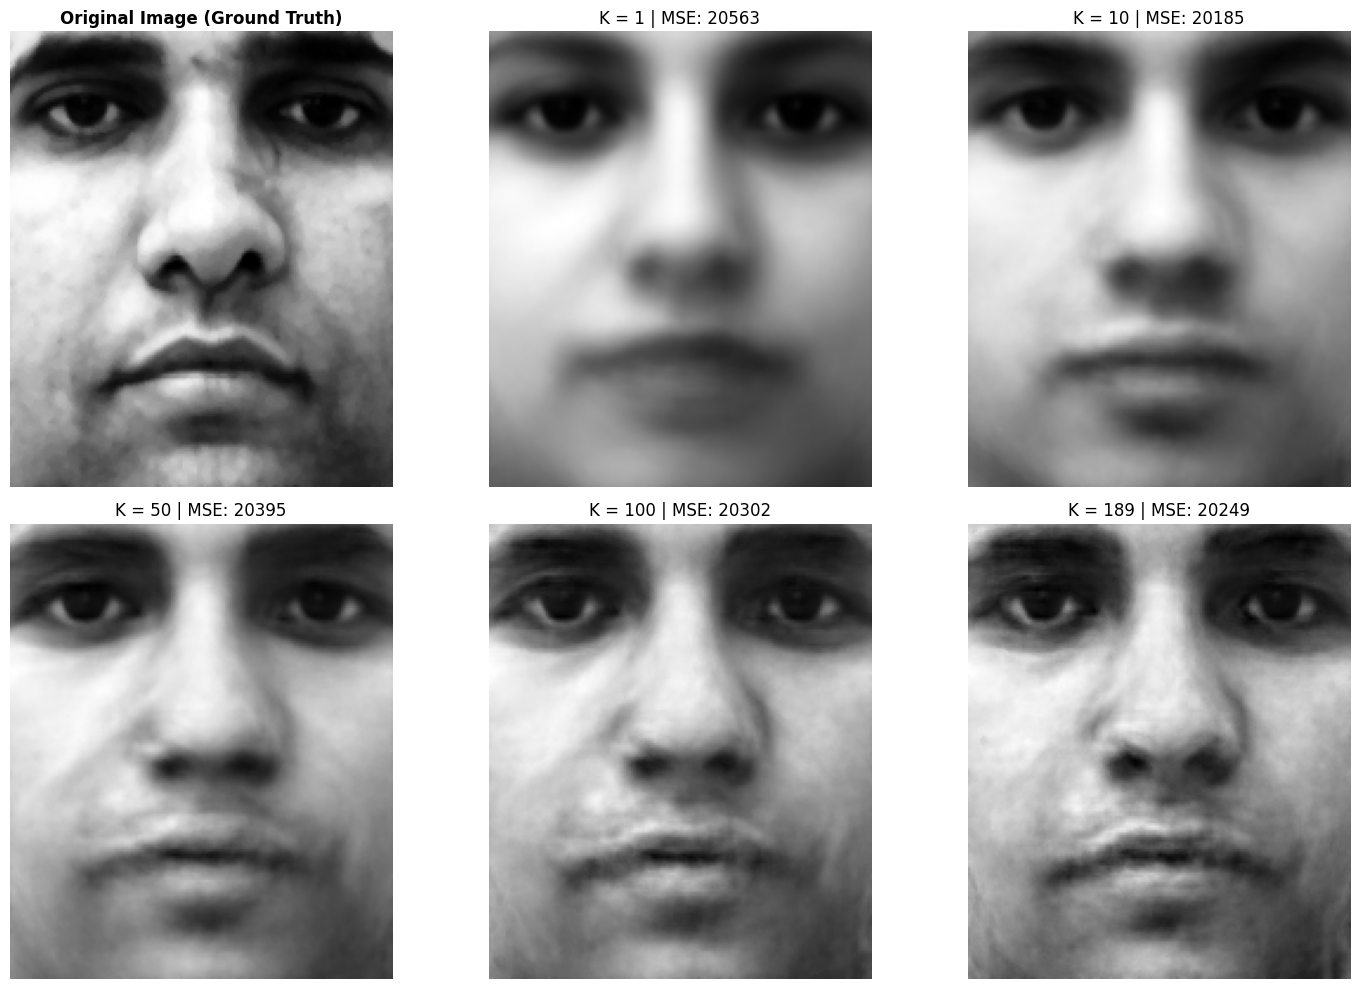
\includegraphics[width=.9\textwidth]{images/recon_grid_test.png}
\captionof{figure}{بازسازی موفقیت‌آمیز تصویر فردی که در مجموعه داده‌های آموزش حضور نداشته است}
\label{fig:recon_grid_test}
\end{center}
}

\field{۸. چالش بازسازی تصاویر غیرانسانی \lr{(Non-human Images)}}{
برای بررسی درک الگوریتم از مفهوم «چهره»، تصاویری از یک عقاب و یک ماشین به سیستم داده شد. از آنجا که پایه و اساس مدل ما ($U_K$) تنها از ویژگی‌های صورت انسان (چشم، بینی انسان و ...) تشکیل شده است، الگوریتم به صورت جبری تلاش می‌کند تا تصویر ماشین را با ترکیب اجزای صورت انسان بسازد! نتیجه‌ی این کار، تولید تصاویری شبح‌مانند و بسیار نامفهوم با خطای \lr{MSE} به شدت بالا بود. این آزمایش به وضوح نشان داد که فضای \lr{PCA} ساخته‌شده، کاملاً به دامنه داده‌های آموزش \lr{(Domain-Specific)} محدود است.

\vspace{0.4cm}
\begin{center}
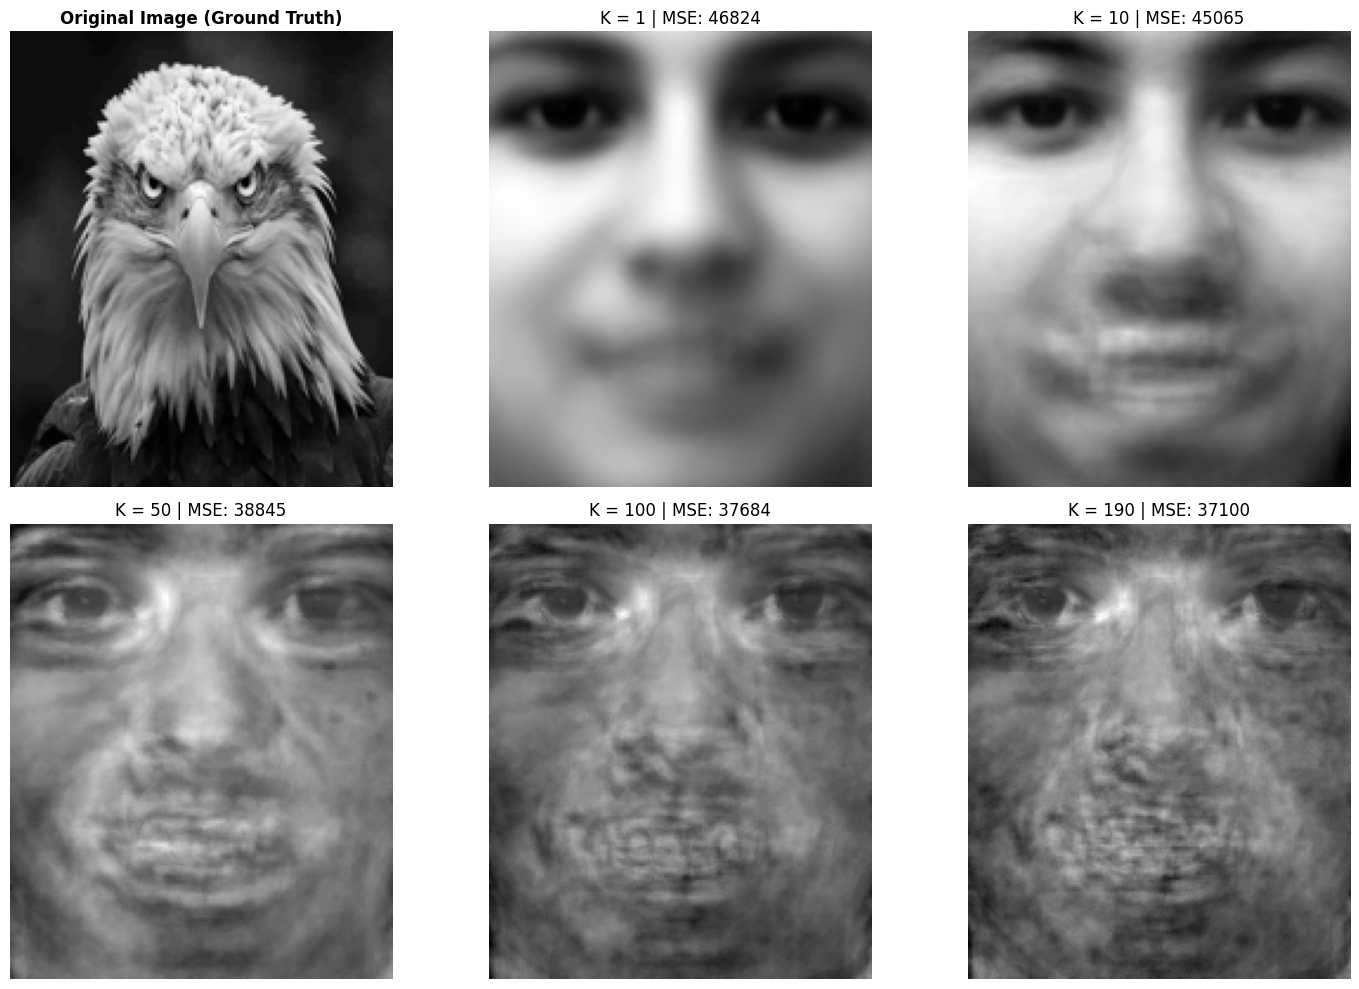
\includegraphics[width=.9\textwidth]{images/recon_grid_nonhuman.png}
\captionof{figure}{تلاش الگوریتم برای بازسازی تصویر غیرانسانی با استفاده از چهره‌های پایه‌ی انسانی}
\label{fig:recon_grid_nonhuman}
\end{center}
}

\field{۹. چالش مقاومت در برابر چرخش \lr{(Rotation Vulnerability)}}{
بزرگترین نقطه‌ضعف الگوریتم‌های مبتنی بر فلت کردن \lr{(Flattening)} تصاویر، عدم مقاومت آن‌ها در برابر تغییرات هندسی مانند چرخش است. برای اثبات این موضوع، یک تصویر از ۰ تا ۳۶۰ درجه (با گام‌های مشخص) دوران داده شد و خطای بازسازی آن اندازه‌گیری گردید.

همان‌طور که در نمودار زیر مشاهده می‌شود، در زوایای ۰ و ۳۶۰ درجه خطا در کمترین حالت خود قرار دارد. اما با نزدیک شدن به زاویه ۱۸۰ درجه (تصویر سر و ته)، خطای \lr{MSE} به یک قله‌ی بزرگ می‌رسد. از نظر منطقی، با چرخش ۱۸۰ درجه‌ای، پیکسل‌های مربوط به موی سر دقیقاً روی مختصاتی قرار می‌گیرند که الگوریتم انتظار دیدن فک و چانه را دارد. 

\vspace{0.4cm}
\begin{center}
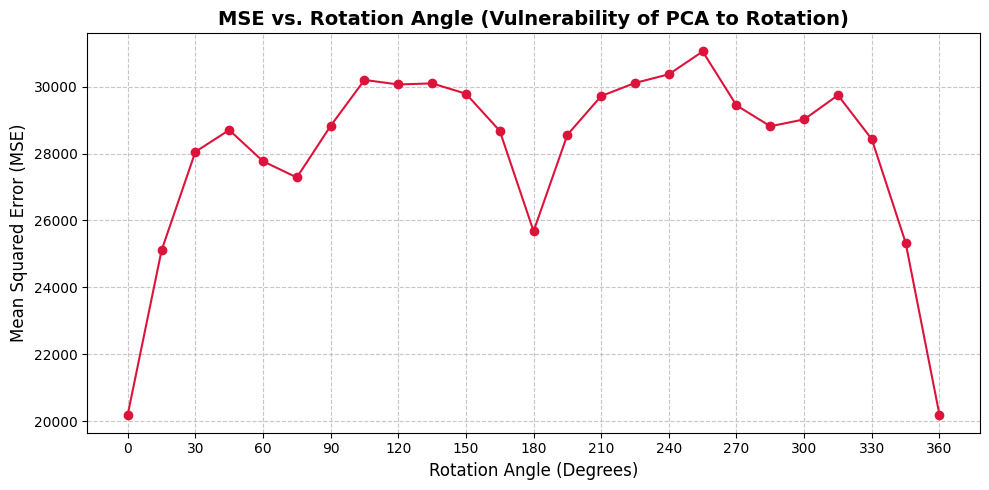
\includegraphics[width=.6\textwidth]{images/rotation_mse.png}
\captionof{figure}{نمودار افزایش شدید خطای \lr{MSE} در اثر چرخش تصویر (عدم مقاومت در برابر چرخش)}
\label{fig:rotation_mse}
\end{center}

برای نمایش بصری این فاجعه‌ی محاسباتی، تصاویر اصلی، چرخش‌یافته و بازسازی‌شده در زوایای مختلف به صورت زیر رسم شدند. این آزمایش دلیل اصلی عبور جامعه‌ی هوش مصنوعی از الگوریتم \lr{PCA} برای پردازش تصویر و روی آوردن به شبکه‌های عصبی پیچشی \lr{(CNN)} را توجیه می‌کند.

\vspace{0.4cm}
\begin{center}
    
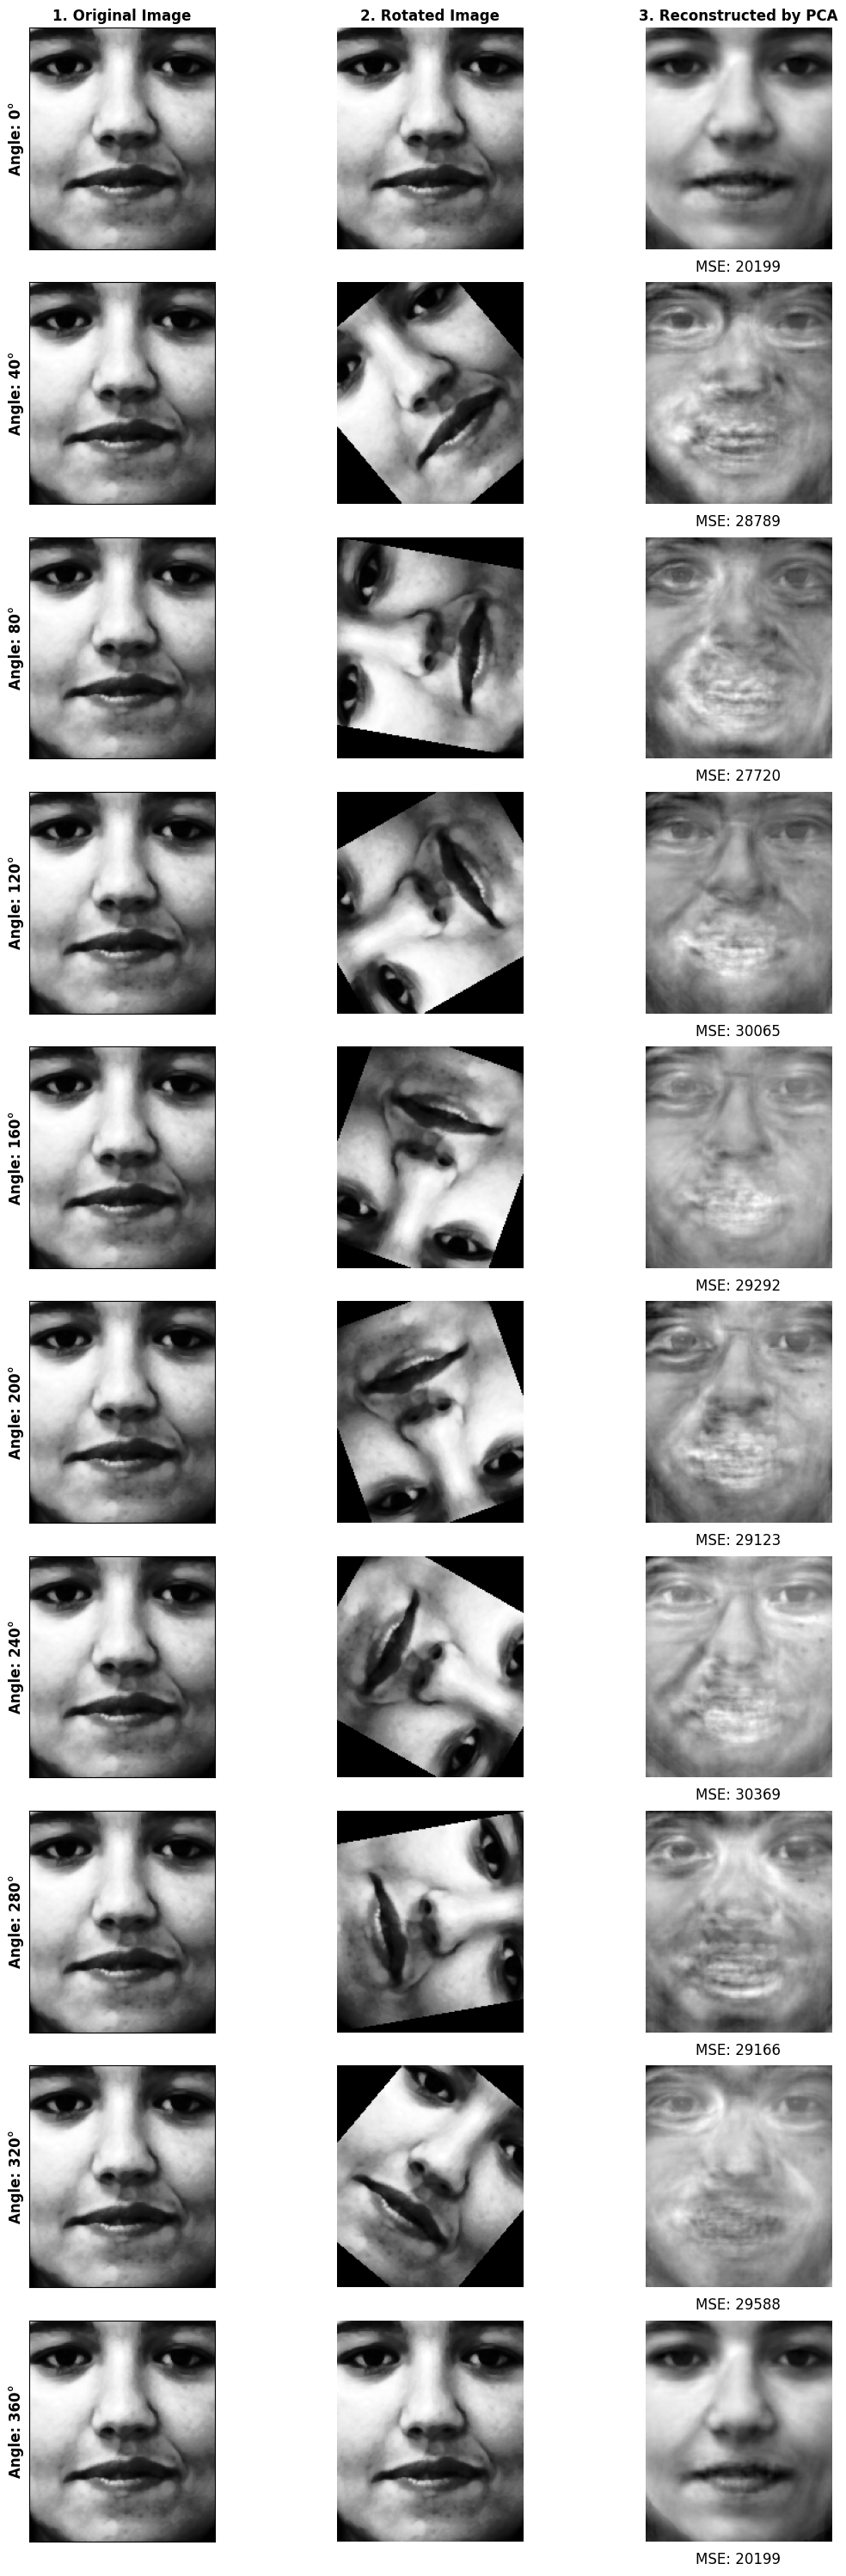
\includegraphics[height=0.75\textheight, keepaspectratio]{images/rotation_grid.png}
\captionof{figure}{گرید بررسی تحلیلی روند شکست الگوریتم در بازسازی تصاویرِ دوران‌یافته}
\label{fig:rotation_grid}
\end{center}
}

\end{stepbox}